%%%%%%%%%%%%%%%%%%%%%%%%%%%%%%%%%%%%%%%%%%%%%%%%%%%%%%%%%%%%%%%%%%%%%%
%%                           CHAPTER 3
%%%%%%%%%%%%%%%%%%%%%%%%%%%%%%%%%%%%%%%%%%%%%%%%%%%%%%%%%%%%%%%%%%%%%

\chapter{\uppercase {\textbf{Chapter 3 - Methodology}}}

This chapter presents the research design, development methodology, system architecture, feature extraction process, model development process, Android deployment plan, testing procedure, and evaluation method used in the development of VoxGest. The methodology is written to explain what was developed, why each approach was selected, and how each component is implemented in relation to the objectives of the study.

\section{Research Design}

This study uses a developmental research design. Developmental research is appropriate because the study focuses on the creation, improvement, and evaluation of a working technology artifact. The output of the study is not limited to theoretical analysis; it includes the design and development of VoxGest as an Android-based assistive communication prototype.

The system was developed to address a practical communication problem between sign language users and hearing or non-signing individuals. The research process therefore includes requirement analysis, system design, machine learning model development, live recognition testing, Android handoff preparation, and software quality evaluation. The system will be evaluated using ISO/IEC 25010 quality characteristics, specifically Functional Suitability, Performance Efficiency, Reliability, and Usability.

\section{Development Methodology}

The development of VoxGest follows Agile Rapid Application Development. This methodology was selected because the project requires continuous testing, revision, and refinement. Sign language recognition systems are sensitive to camera quality, lighting, background, hand visibility, motion timing, body position, and differences between saved training data and live usage. A strictly linear development process would not be suitable because the system must be tested repeatedly in real camera conditions.

The Agile RAD process used in VoxGest consists of the following phases:

\begin{enumerate}
    \item Brainstorming and problem identification;
    \item Requirement analysis and scope definition;
    \item Dataset preparation and sample collection;
    \item Feature extraction and preprocessing;
    \item Model development and export;
    \item Live recognition testing and hardening;
    \item Android prototype integration;
    \item Evaluation preparation; and
    \item Documentation and research paper refinement.
\end{enumerate}

This iterative approach allowed the researchers to improve the system when earlier models showed weaknesses. The project initially explored image-based CNN recognition, then attempted a hybrid image-and-landmark approach, and later shifted toward landmark-based static recognition and temporal dynamic recognition because these approaches matched the live camera requirements more effectively.

\section{System Architecture}

VoxGest is designed as an offline Android edge-computing accessibility system. The general system flow is:

\begin{center}
\texttt{camera input -> landmarks -> static/dynamic model -> gates -> token composer -> text/speech/avatar}
\end{center}

The system begins with camera input from the Android device. Frames are processed through a landmark extraction pipeline. Static signs are passed to the static alphabet recognition model, while dynamic words are passed to the temporal word recognition model. Predictions are not immediately accepted; they are filtered through confidence, margin, motion, wrist path, hand presence, stability, and cooldown rules. Accepted predictions are passed to the token composer, which builds the final text output. The text can then be displayed, spoken through text-to-speech, or passed to the avatar module.

For the reverse communication direction, the hearing user can speak into the application. The speech-to-text module converts the spoken reply into text. Known words may trigger avatar animations, while unknown words can be fingerspelled. This creates a bidirectional communication flow between the signing user and the hearing or non-signing user.

\begin{figure}[h!]
\centering
    \centerline{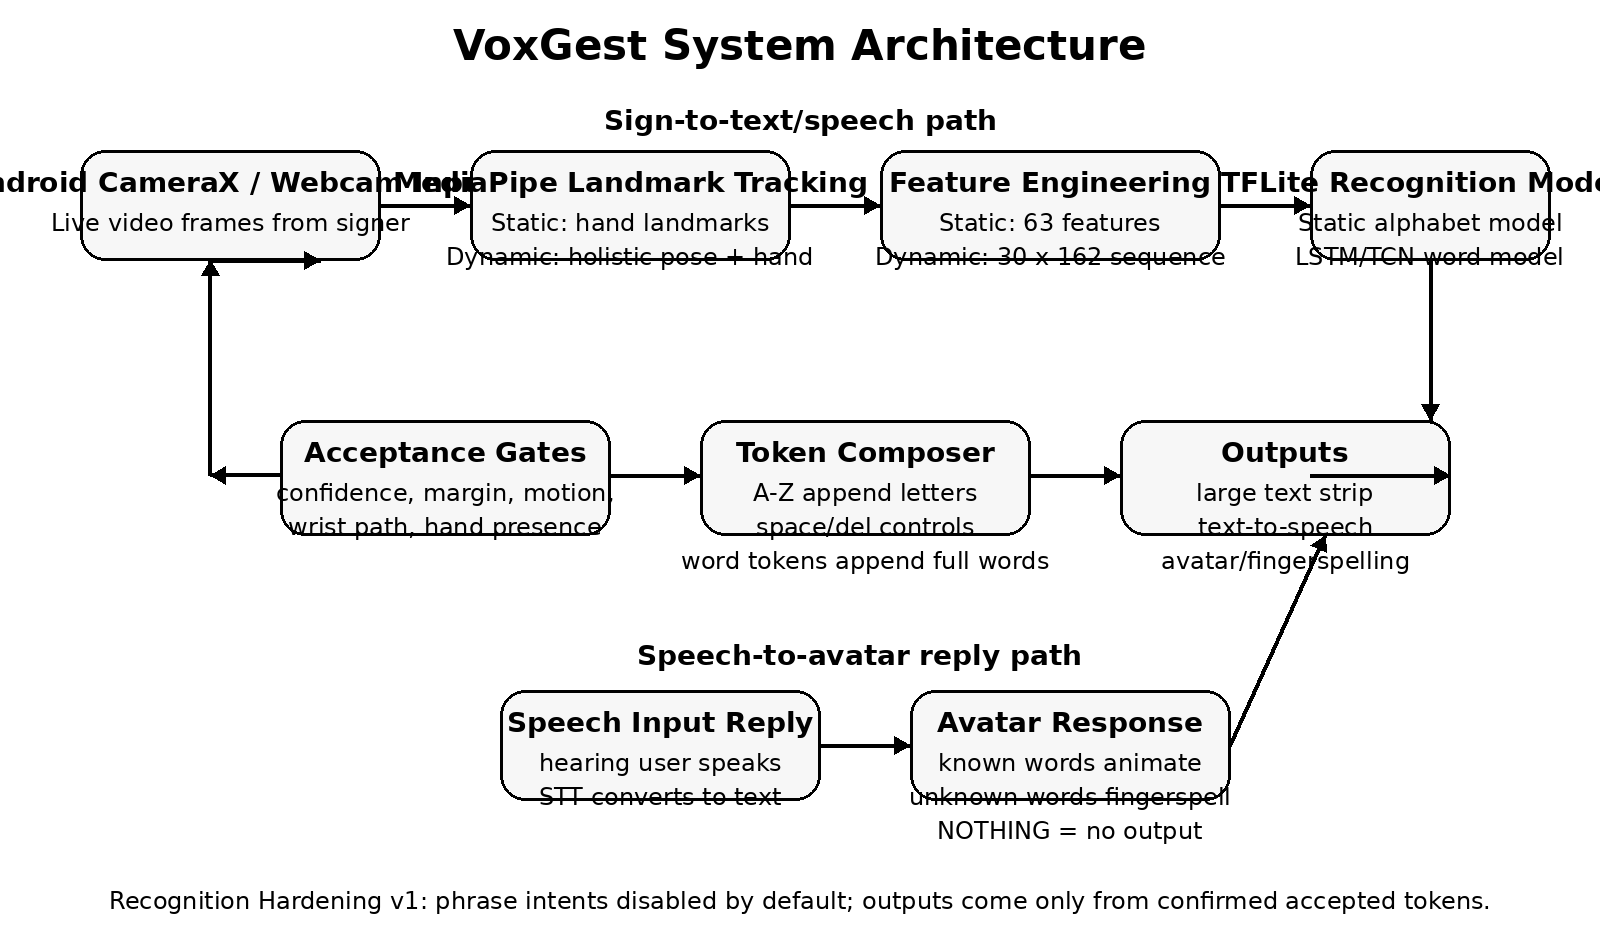
\includegraphics[width=0.95\textwidth]{figures/Fig3.1.png}}
    \caption{VoxGest System Design Architecture}
\end{figure}

\section{System Components}

The VoxGest system is composed of the following components:

\begin{enumerate}
    \item \textbf{Camera Input Module} - captures live video frames from the Android camera or webcam prototype.
    \item \textbf{Landmark Extraction Module} - extracts hand and pose landmarks using MediaPipe-based tracking.
    \item \textbf{Static Alphabet Recognition Module} - recognizes A-Z, del, space, and nothing using 63 hand-landmark features.
    \item \textbf{Dynamic Word Recognition Module} - recognizes selected motion words using 30-frame sequences with 162 features per frame.
    \item \textbf{Post-Processing and Acceptance Module} - prevents unstable predictions using thresholds, smoothing, gates, and cooldown rules.
    \item \textbf{Token Composer Module} - builds message text only from confirmed accepted letters, controls, and word tokens.
    \item \textbf{Text-to-Speech Module} - speaks confirmed recognized output for the hearing or non-signing user.
    \item \textbf{Speech-to-Text Module} - captures spoken replies and converts them into readable text.
    \item \textbf{Avatar and Fingerspelling Module} - provides visual feedback using known word animations or fingerspelling fallback.
\end{enumerate}

\section{Dataset Development}

The dataset development process was divided into static alphabet data, dynamic word data, negative/no-output data, and future phrase-intent data.

\subsection{Static Alphabet Dataset}

The static alphabet dataset was prepared for A-Z, del, space, and nothing. The first version of the project used image datasets for CNN-based recognition. However, live testing showed that image-based recognition did not generalize well under webcam conditions. For this reason, the project moved toward a landmark-based dataset where each sample represents the geometry of the hand instead of the entire image.

For static recognition, each hand sample contains 21 landmarks with x, y, and z coordinates. This produces 63 numerical features. The model is trained to classify these features into static alphabet and control labels.

\subsection{Dynamic Word Dataset}

The dynamic dataset contains selected word signs that require movement over time. The active dynamic labels are YES, NO, PLEASE, WATER, HELLO, HELP, STOP, DOCTOR, NAME, THANKYOU, and NOTHING. Each dynamic sample is represented as a 30-frame sequence. Each frame contains pose and dominant-hand features so the model can understand both hand motion and body-relative location.

Dynamic samples may come from selected videos, WLASL-related sources, and manual webcam calibration recordings. Live calibration is important because a model trained only on external videos may not match the actual camera, signer, angle, lighting, and motion style used in the application.

\subsection{Negative and No-Output Samples}

The NOTHING class is collected as a negative class. It includes idle hands, relaxed hands, open hands, hand entering or leaving the frame, transition movements, partial signs, aborted signs, and neutral non-sign movement. NOTHING is not a word token. It is used to reduce false outputs by teaching the model when no valid sign should be displayed, spoken, or animated.

\section{Feature Engineering}

Feature engineering converts camera-based visual input into numerical data that can be processed by the recognition models.

\subsection{Static Feature Engineering}

For static alphabet recognition, the system uses 21 hand landmarks. Each landmark has x, y, and z coordinates:

\begin{center}
\texttt{21 landmarks x 3 coordinates = 63 features}
\end{center}

The static feature vector is normalized by subtracting the wrist landmark from every point and scaling the hand using a stable hand-size reference. This makes the same sign more consistent even when the hand is closer, farther, or slightly shifted in the camera view.

\subsection{Dynamic Feature Engineering}

For dynamic word recognition, the system uses a 30-frame temporal sequence. Each frame contains:

\begin{center}
\texttt{33 pose landmarks x 3 = 99 features} \\
\texttt{21 dominant-hand landmarks x 3 = 63 features} \\
\texttt{99 + 63 = 162 features per frame}
\end{center}

The dynamic model input is therefore:

\begin{center}
\texttt{[1, 30, 162]}
\end{center}

The pose and hand features are anchored to the pose nose point to provide body-relative context. This design helps differentiate signs that may have similar hand shape or movement but occur in different body locations. The system also supports a strict single-hand feature policy that keeps the head, torso, selected arm, and selected hand while masking non-dominant arm and unrelated lower-body landmarks.

\section{Model Development}

\subsection{Initial CNN Approach}

The first model approach used a CNN trained on static ASL alphabet images. This was selected because CNNs are commonly used for image recognition and can learn visual patterns from raw images. However, live webcam testing revealed that image-based recognition was sensitive to background, lighting, cropping, camera distance, and dataset mismatch. The CNN approach is therefore documented as an early research iteration rather than the final system approach.

\subsection{Hybrid CNN and Landmark Attempt}

A hybrid model was later considered to combine raw image features with hand landmark features. This was intended to help distinguish visually similar signs. However, the approach introduced more preprocessing complexity and remained vulnerable to image-branch problems. Because the goal of the project is reliable real-time mobile recognition, the system shifted toward a simpler and more controllable landmark-based pipeline.

\subsection{Landmark-Based Static Model}

The current static recognition approach uses normalized 63-feature hand landmarks. This was chosen because hand landmarks reduce background and lighting dependence and make the Python and Android pipelines easier to align. The static model recognizes A-Z, del, space, and nothing.

\subsection{Dynamic LSTM and TCN Models}

The dynamic word model uses temporal sequence learning because dynamic signs are defined by motion over time. LSTM is used because it can learn sequence order and motion dependencies. TCN is also considered because temporal convolution can be efficient for sequence modeling and may perform well in mobile deployment. VoxGest compares model behavior using both validation results and live camera tests.

The dynamic model currently uses a 30-frame input with 162 features per frame and recognizes the current 10-word vocabulary plus NOTHING. The current dynamic recognition stage is considered recognition hardening, meaning that the project prioritizes improving the existing vocabulary before adding more signs.

\section{Recognition Hardening and Post-Processing}

Recognition hardening is the process of improving live reliability after model training. The system does not immediately trust a raw prediction. Instead, it checks whether a prediction is confident, stable, and supported by enough motion and hand presence.

The post-processing gates include:

\begin{enumerate}
    \item \textbf{Confidence} - the probability score of the predicted class;
    \item \textbf{Margin} - the separation between the top prediction and the next likely class;
    \item \textbf{Motion Energy} - whether enough movement occurred for a dynamic word;
    \item \textbf{Wrist Path} - whether the hand traveled enough distance during the sequence;
    \item \textbf{Hand Presence} - whether the configured hand was visible enough during the sequence;
    \item \textbf{Stable Frames} - whether the prediction remains consistent across multiple frames; and
    \item \textbf{Cooldown} - a waiting period that prevents repeated duplicate outputs.
\end{enumerate}

These gates are important because the model may otherwise produce random words during idle hands, partial signs, or camera jitter. The NOTHING class and the acceptance gates work together to prevent unstable predictions from becoming text, speech, or avatar output.

\section{Android Application Development}

The Android application is designed to consume exported model files and perform on-device inference. The recommended Android stack includes Kotlin, CameraX for camera preview and frame analysis, MediaPipe Holistic or an equivalent landmark pipeline, and TensorFlow Lite Interpreter for static and dynamic models.

The Android application should provide the following screens and features:

\begin{enumerate}
    \item Camera permission and startup screen;
    \item Live recognition screen;
    \item Recognition mode switch for AUTO, LETTERS, and WORDS;
    \item Large current prediction display;
    \item Text strip for recognized output;
    \item Clear or delete controls;
    \item Optional debug metrics for development builds;
    \item Speech output for confirmed tokens;
    \item Speech-to-text input for hearing-user replies; and
    \item Avatar or fingerspelling response panel.
\end{enumerate}

The Android app must match the Python preprocessing rules. If Android selects a different hand, mirrors the camera differently, or normalizes landmarks differently, the same sign may become a different model input. Therefore, Python and Android must share the same input shapes, label order, landmark normalization, dominant-hand policy, and post-processing thresholds.

\section{Avatar and Speech Communication Module}

The text-to-speech module speaks confirmed recognized text so the hearing or non-signing user can understand the sign language user's input. The speech-to-text module allows the hearing user to respond through spoken language, which is converted into readable text.

The avatar module provides a visual response for the signing user. Known words can trigger lightweight animation files, while unknown words can be fingerspelled. The avatar is downstream of the token composer. This means raw predictions, rejected predictions, and unstable predictions must not trigger avatar animation. Only confirmed accepted tokens should be passed to the avatar.

The current avatar module is a prototype. It does not claim full ASL grammar generation. Its role is to provide basic visual feedback for the controlled demo vocabulary and to show the feasibility of a bidirectional communication interface.

\section{Testing Procedure}

Testing is divided into static testing, dynamic testing, negative/no-output testing, Android readiness testing, and user evaluation preparation.

\subsection{Static Recognition Testing}

Static recognition testing checks whether A-Z, del, space, and nothing can be recognized reliably. The researchers use live alphabet testing and diagnostic tools to identify weak static signs. When weak signs are found, additional static calibration samples may be recorded and used to retrain the static landmark model.

\subsection{Dynamic Word Testing}

Dynamic testing checks whether the current 10 word signs can be recognized in live camera conditions. The system records confidence, margin, motion, wrist path, hand presence, accepted or rejected status, and confusion cases. This helps the researchers determine whether a word needs additional samples, threshold tuning, or cleaner metadata.

\subsection{Negative Class Testing}

Negative testing verifies whether the system rejects idle hands, open hands, partial signs, transition movement, and aborted signs. These samples are treated as NOTHING. Successful negative-class behavior means that the system does not produce a random word when the user is not signing a valid word.

\subsection{Android Readiness Testing}

Android readiness testing verifies whether the exported model files, label files, runtime manifest, and feature rules can be integrated into the Android prototype. The Android developer must follow the same feature extraction and inference contract used in the Python prototype.

\section{Evaluation Method}

The completed VoxGest prototype will be evaluated using selected ISO/IEC 25010 quality characteristics. The criteria are Functional Suitability, Performance Efficiency, Reliability, and Usability.

\begin{enumerate}
    \item \textbf{Functional Suitability} evaluates whether VoxGest performs its required communication functions, including recognition, text output, speech output, speech-to-text, and avatar response.
    \item \textbf{Performance Efficiency} evaluates whether the system responds fast enough for real-time communication and runs suitably on mobile hardware.
    \item \textbf{Reliability} evaluates whether the system produces stable outputs, handles missing landmarks, and reduces false recognition.
    \item \textbf{Usability} evaluates whether the interface is understandable and usable by target users and evaluators.
\end{enumerate}

\section{Respondents of the Study}

The study will involve two main respondent groups. IT professionals will evaluate the technical quality of the system, including functionality, performance, reliability, and implementation feasibility. Deaf, mute, hard-of-hearing, signing users, or representative users will evaluate usability, communication effectiveness, readability, accessibility, and user experience.

The final number of respondents may depend on availability and adviser approval. The recommended minimum target is to include IT professionals for technical evaluation and target or representative users for accessibility and usability evaluation.

\section{Data Gathering Instrument}

The main data gathering instrument will be a structured questionnaire based on ISO/IEC 25010. The questionnaire will use a 5-point Likert scale.

\begin{table}[h!]
\caption{Likert Scale Interpretation}
\vspace{-1em}
\begin{center}
\begin{tabular}{|| c c c ||} 
 \hline
 Weight & Range & Interpretation \\ [0.5ex] 
 \hline\hline
 5 & 4.50 - 5.00 & Excellent / Strongly Agree \\ 
 \hline
 4 & 3.50 - 4.49 & Very Good / Agree \\ 
 \hline
 3 & 2.50 - 3.49 & Good / Neutral \\ 
 \hline
 2 & 1.50 - 2.49 & Fair / Disagree \\ 
 \hline
 1 & 1.00 - 1.49 & Poor / Strongly Disagree \\ [1ex] 
 \hline
\end{tabular}
\end{center}
\end{table}

The questionnaire items will be grouped according to Functional Suitability, Performance Efficiency, Reliability, and Usability. Additional comments may also be collected to gather qualitative suggestions for improvement.

\section{Statistical Treatment of Data}

The evaluation results will be analyzed using descriptive statistics. The weighted mean will be used to summarize the responses for each ISO/IEC 25010 category. The formula for the weighted mean is:

\begin{center}
\texttt{Weighted Mean = Sum of weighted responses / Total number of responses}
\end{center}

The computed mean for each category will be interpreted using the Likert scale table. This will allow the researchers to determine the overall acceptability and software quality of the VoxGest prototype.

\section{Research Ethics}

The researchers will ensure that respondents are informed about the purpose of the study, the testing activity, and the use of their feedback. Participation will be voluntary. Respondents may decline or stop participation at any time. Any collected responses will be used only for academic evaluation. If images, videos, or demonstration recordings are collected, the researchers will request consent and avoid publishing personally identifiable data without permission.

Because VoxGest involves camera-based input and accessibility-related users, privacy and respect are important. The system is designed for local recognition, and the recognition prototype does not require cloud processing for the current scope.

\section{Summary of Methodology}

This chapter explained the methodology used in the development of VoxGest. The study uses developmental research and Agile Rapid Application Development because the project involves building, testing, and improving a working assistive communication system. The current system architecture uses camera input, MediaPipe landmark extraction, static and dynamic recognition models, post-processing gates, token composition, text output, text-to-speech, speech-to-text, and avatar or fingerspelling response.

The methodology also explained why the project evolved from CNN-based image recognition to landmark-based and temporal recognition. Static signs use 63 hand-landmark features, while dynamic words use 30-frame sequences with 162 pose and dominant-hand features per frame. The NOTHING class, dominant-hand policy, and post-processing gates are included to support reliability and reduce false outputs. The completed prototype will be evaluated using ISO/IEC 25010 quality characteristics through questionnaires answered by IT professionals and target or representative users.
